% !Mode:: "TeX:UTF-8"

\chapter[基于深度学习的语义依存图分析]{基于深度学习的语义依存图分析}[Semantic Dependency Graph Parsing Based on Deep Learning]

\section{引言}[Introduction]

在过去的二十几年中,自然语言处理领域涌现出了大量的关于树结构的句法分析的研究工作\cite{eisner-1996-three, nivre-2004-incrementality, mcdonald-etal-2006-online, nivre-2009-non, zhang-nivre-2011-transition}。
近年来,在神经网络模型的帮助下,句法依存分析的准确率取得了显著的提升\cite{chen-manning-2014-fast,weiss-etal-2015-structured, andor-etal-2016-globally}。
然而,当表示的目标从句法结构变为深层语义结构时,树结构的不足之处就展现了出来。
从语义层面上来说,句子中的一个词可以同时作为多个谓词(predicate)的论元(argument)。
为了刻画这种语义关系,有研究者使用了有向无环图(a directed acyclic graph,简称DAG)结构,其中的节点允许有多条入弧。
Oepen等人\cite{oepen-etal-2015-semeval}于2015年公布了Broad-Coverage Semantic Dependency Graph语料库,包含了英文、捷克语和中文上的三种语义依存图标注。
而Che等人\cite{che-etal-2016-semeval}于2016年公布了中文语义依存图语料库。
本文重点研究的就是其中的中文语义依存图的分析技术及应用。

正如第\ref{sec:sdp}节所介绍,图结构的引入在提升语义表示能力的同时,也因其中每个词父节点数量的不确定性给依存图分析带来了巨大的挑战。
虽然语义依存图的分析方法可以从其前身——句法依存树分析的工作中寻找灵感,但如何生成多父节点词,是所有的依存图分析方法都无法回避的,也是依存图分析中的核心问题。
除此之外,此前的语义依存图分析模型,大部分仍然在使用传统的基于特征工程的统计机器学习方法。
然而自从Chen等人\cite{chen-manning-2014-fast}于2014年首次将神经网络模型引入基于转移的句法依存分析器中,神经网络模型已经在依存分析领域证明了其强大的特征表示能力。
但该方法仍然使用了人工设计的特征,没有完全避免需要专家知识的特征工程。

总的来说,想要实现高效、准确的语义依存图分析模型需要面临两个挑战:

1.如何解决多父节点词的问题?

2.如何更高效、准确地实现分析模型的学习?

针对上述第一个问题,本章采用了基于转移的分析方法,设计了一套用于生成依存图的转移系统,使其在不需要预处理和后处理的情况下能够直接根据输入的句子完整地生成其对应的语义依存图。

针对上述第二个问题,本章采用了基于栈-长短时记忆网络(Stack-LSTM)的模型,用LSTM分别获取转移系统中各个部分的上下文相关表示向量,组成当前转移状态的表示向量,并用其预测下一个转移动作。
特别的,本章为转移系统中重要的队列和已经生成的子图分别使用了双向LSTM相减模块和递增的Tree-LSTM模块来更好地获取其表示。

本章在前文介绍的中文和英文的语义依存图语料库上分别测试了上述模型,实验结果表明,本章提出的语义依存图分析方法在此前方法的基础上取得了显著的性能提升。

\section{背景与相关工作}[Related Work]
\label{sec:chapter2-related-work}

基于转移的依存分析主要由转移系统和转移动作分类器两部分组成。
其中转移系统包括了由列表、栈等结构组成的环境和一系列预定义的对环境进行改变的转移动作。
包括列表、栈等结构在内的所有环境在某一时间节点的情况称为转移状态。
转移动作在执行时不仅修改转移状态,也会同时生成词之间的依存弧,而目标依存结构就是通过一系列的转移动作生成的。
本文第\ref{sec:syntactic-dependency-parsing}节已经介绍了标准弧转移系统并简要介绍了基于转移的分析模型中的转移动作分类器。
本节将重点介绍与本章研究内容密切相关的贪心弧转移系统(Arc-Eager Transition System)\cite{choi-palmer-2011-getting,choi-mccallum-2013-transition}和Stack-LSTM模型结构\cite{dyer-etal-2015-transition}。

Choi等人\cite{choi-palmer-2011-getting}于2011年提出了一种贪心弧转移算法。
从转移动作上来说,该算法与标准弧转移算法的主要区别是标准弧转移算法生成的是栈顶的两个词之间的依存关系,而贪心弧转移算法生成的是栈顶词和列表中第一个词之间的依存关系。
这种生成弧的顺序无法保证一个词找到其父节点时其所有子节点都已经提前找到,为了解决这一问题,该算法里又增加了规约(Reduce)和跳过(PASS)动作。
其中规约动作用于处理所有入弧和出弧都已经找到的节点,将其从转移状态中删除。
有了规约动作,原来生成弧的动作,即左弧(Left)和右弧(Right)将不再承担删除子节点的任务。
而跳过动作则暂时将栈顶词弹出,从而允许列表中的词与栈中其他词之间生成弧。
而为了保存栈顶弹出的词,该算法的转移状态中在一般的栈和列表的基础上额外增加了一个双向队列,专门保存这些被弹出的词,等到下一个移进动作时一起再移入栈中。

从另一个角度来说,这种转移动作的设计实际上是通过将生成弧的动作与删除词的动作分离来解决贪心弧转移算法的劣势,即生成弧的时候无法保证该弧指向的子节点的所有子节点都已经找到。
然而这种转移动作的分离又引入了一个新的问题。
基于转移的依存分析方法中,转移动作分类器通过当前转移状态来预测下一个要执行的转移动作,这就要求每个转移动作执行之后会对转移状态进行明显的修改。
然而由于生成弧的动作不再删除子节点,其对转移状态的改变很小(只是在已生成的子图中加了一条弧),难以被分类器察觉。
为了解决这一问题,Choi等人对生成弧的动作(包括左弧、右弧和不生成弧)和修改转移状态的动作(移进、规约等)进行了组合,确保每个生成弧的动作都会对转移状态进行修改。

\begin{table}[htbp]
	\centering
	%\small
	%\renewcommand{\arraystretch}{1.2}
	\begin{tabular}{l|ll}
		\hline
		\bf 转移动作 \ \ \ \ & \bf 当前转移状态 & $\Rightarrow$ \bf 下一转移状态 \\
		\hline\hline
		Left$_l$-Reduce &\ \ $([\sigma|i],\,\delta,\,[j|\beta],\,E)$ & $\Rightarrow (\sigma,\,\delta,\,[j|\beta],\,E\,\cup\,\{(i\xleftarrow{l}j)\})$ \\
		Right$_l$-Shift &\ \ $([\sigma|i],\,\delta,\,[j|\beta],\,E)$ & $\Rightarrow ([\sigma|i|\delta|j],\,[\ ],\,\beta,\,E\,\cup\,\{(i\xrightarrow{l}j)\})$ \\
		No-Shift &\ \ $([\sigma|i],\,\delta,\,[j|\beta],\,E)$ & $\Rightarrow 
		([\sigma|i|\delta|j],\,[\ ],\,\beta,\,E)$ \\
		No-Reduce &\ \ $([\sigma|i],\,\delta,\,[j|\beta],\,E)$ & $\Rightarrow (\sigma,\,\delta,\,[j|\beta],\,E)$\\
		\hline
		Left$_l$-Pass &\ \ $([\sigma|i],\,\delta,\,[j|\beta],\,E)$ & $\Rightarrow (\sigma,\,[i|\delta],\,[j|\beta],\,E\,\cup\,\{(i\xleftarrow{l}j)\})$\\
		Right$_l$-Pass &\ \ $([\sigma|i],\,\delta,\,[j|\beta],\,E)$ & $\Rightarrow (\sigma,\,[i|\delta],\,[j|\beta],\,E\,\cup\,\{(i\xrightarrow{l}j)\})$\\
		No-Pass &\ \ $([\sigma|i],\,\delta,\,[j|\beta],\,E)$ & $\Rightarrow (\sigma,\,[i|\delta]	,\,[j|\beta],\,E)$\\
		\hline
	\end{tabular}
	\bicaption[tbl:choi-transition-actions]{}{List-Based Arc-Eager转移算法中的转移动作集合}{Table$\!$}{Transition actions in List-Based Arc-Eager transition algorithm.}
	\label{tbl:actions}
\end{table}

他们将该算法命名为基于列表的贪心弧(List-Based Arc-Eager)转移算法,其中定义的转移动作如表\ref{tbl:choi-transition-actions}所示。
表中$\sigma$,$\delta$和$\beta$分别代表上文介绍的转移系统中的栈、双向队列和列表。
而$E$表示算法生成的所有依存弧集合。

值得注意的是,将生成弧的动作和删除词的动作进行分离的思想,虽然在该工作中是为了弥补贪心弧转移算法的劣势,但对于语义依存图的生成也有重要意义。
利用这种思想可以设计出适用于依存图生成的转移系统,在为句中词找到一个父节点的时候不立即将其从转移状态中删除,而是继续寻找它的其他父节点,直到一个词的所有父节点都已找到再对其进行规约。
因此,本章选择在List-Based Arc-Eager转移算法的基础上设计语义依存图的转移算法。

% stack-lstm
Chen等人\cite{chen-manning-2014-fast}于2014年首次将多层感知器(
Multi-Layer Perceptron,简称MLP)引入基于转移的依存分析器,利用其强大的表示能力显著提高了句法依存分析的性能。
但该方法仍然受限于传统特征工程的思想,使用了固定位置的隐层表示作为转移状态的表示,用于预测下一个转移动作。
尽管如此,该方法开启了基于神经网络模型的句法依存分析的大门,启发了此后很多的相关工作。

Dyer等人\cite{dyer-etal-2015-transition}于2015年提出了使用Stack-LSTM代替MLP,从而全自动地获取转移状态表示的方法。
具体来说,假设$\bm{x}_t$是$t$时刻的输入向量,普通的LSTM在$t$时刻首先计算控制信息的输入门$\bm{i}_t$(Input Gate)、遗忘门$\bm{f}_t$(Forget Gate)和保存信息的记忆单元$\bm{c}_t$(Memory Cell):
\begin{equation}
    \bm{i}_t = \sigma(\bm{W}_{ix}\bm{x}_t + \bm{W}_{ih}\bm{h}_{t-1} + \bm{W}_{ic}\bm{c}_{t-1} + \bm{b}_i)
\end{equation}
\begin{equation}
    \bm{f}_t = \sigma(\bm{W}_{fx}\bm{x}_t + \bm{W}_{fh}\bm{h}_{t-1} + \bm{W}_{fc}\bm{c}_{t-1} + \bm{b}_f)
\end{equation}
\begin{equation}
    \bm{c}_t = \bm{f}_{t}\odot\bm{c}_{t-1} + \bm{i}_{t}\odot \tanh(\bm{W}_{cx}\bm{x}_{t} + \bm{W}_{ch}\bm{h}_{t-1} + \bm{b}_c)
\end{equation}
其中$\odot$表示逐点乘积(Hadamard product),$\sigma$表示非线性变换函数,例如sigmoid或tanh。
之后计算控制LSTM输出的输出门$\bm{o}_t$(Output Gate)并用其计算时刻$t$的隐层输出$\bm{h}_t$:
\begin{equation}
    \bm{o}_t = \sigma(\bm{W}_{ox}\bm{x}_t + \bm{W}_{oh}\bm{h}_{t-1} + \bm{W}_{oc}\bm{c}_{t-1} + \bm{b}_o)
\end{equation}
\begin{equation}
    \bm{h}_t = \bm{f}_{t}\odot\tanh(\bm{c}_{t})
\end{equation}
通过上述三种门的控制和记忆单元,LSTM能够更新、储存和重置较长序列的信息,从而解决长距离依赖问题。

LSTM的特性使其很适合用于抽取基于转移的依存分析器中转移系统各个部分的信息。
然而普通的LSTM只能建模从左到右或从右到左的序列。
而在基于转移的依存分析中,转移系统中的栈中的词是不断变化的,这种变化不仅有单方向的增加,也有删除。
为了解决该问题,Dyer等人提出了Stack-LSTM模型,在普通LSTM中加入一个栈指针,永远指向当前栈顶词。
在从栈中删除栈顶词时,指针指向新的栈顶词。
在向栈中移入新的词时,由栈指针指向的那个词提供LSTM计算所需的$\bm{c}_{t-1}$和$\bm{h}_{t-1}$。
通过这种方式,他们将LSTM成功应用于基于转移的依存分析,实现了全自动的获取当前转移状态的表示,而不需要任何人工定义特征。

本章的提出的语义依存图分析器建立在Stack-LSTM的基础上,并提出了两种神经网络模块,用于更好地获取转移系统中队列和已经生成的子图的表示。


\section{基于转移的语义依存图分析方法}[Transition-Based Semantic Dependency Graph Parsing]

正如第\ref{sec:chapter2-related-work}节所介绍,List-Based Arc-Eager算法中将生成弧的动作和删除词的动作分离的思想,对于依存图的生成也有重要借鉴意义。
因此,为了设计适用于依存图结构的分析器,本章选择了基于转移的分析方法作为突破口,并在List-Based Arc-Eager算法的基础上设计适用于语义依存图生成转移系统。
对于基于转移的分析方法中另一个重要的部分——转移动作分类器,本章选择Stack-LSTM作为基础模型,从而完全摆脱了需要专家知识的特征工程,并为转移系统中重要的保存待处理词的列表和系统中部分生成的子图分别提出了双向LSTM相减模块和递增的Tree-LSTM模块,用以更好地获取其表示。
本节将从转移系统和基于Stack-LSTM的依存图分析器模型结构两方面具体介绍本章提出的语义依存图分析器。
%这类方法通过执行一系列从初始转移状态到终止转移状态的移进、规约等转移动作,实现目标结构的生成。这类方法由两个重要部分组成,一是转移系统,它定义了存放句中词的结构、转移动作集合以及转移动作执行的规则;二是分类器,它以当前转移状态为依据,预测出下一步要执行的转移动作。基于转移的分析方法的核心就是训练一个好的分类器,使得当我们按照它预测的动作产生语义依存图时,与正确的语义依存图尽可能相似。接下来分别介绍我们实现的用于分析语义依存图的转移系统和分类器。

\subsection{转移系统}[Transition System]

%由于语义依存图具有非投射性(弧之间存在交叉),在设计转移系统时,我们参考了Choi等人提出的用于分析非投射依存树的转移系统,\cite{choi-palmer:2011:ACL-HLT2011,choi-mccallum:2013:ACL2013}并对其做了改进,使其能够直接分析语义依存图。
为了处理语义依存图中多父节点词的生成问题,本章在List-Based Arc-Eager算法的基础上设计适用于依存图分析的转移系统。
主要思想是在找到一个词的父节点之后,不再马上将其从转移系统中删除(由于在树结构中,一个词只有一个父节点,因此在分析依存树时,一旦找到了一个词的父节点,就会立即将其从转移系统中删除),而是仍然将其保存在系统中,这样未来这个词就能找到其它的父节点。
要实现这一目的,主要需要对转移系统中各转移动作的执行条件进行更改。
具体来说,基于转移的分析方法的训练过程中首先需要按照预定义的执行条件及正确的语义依存图生成神谕(oracle)转移动作序列。
神谕转移动作序列是一条从初始转移状态一直到终结转移状态的序列,在执行过程中生成正确的语义依存图。
其作用是生成一系列的由当前转移状态到下一步的转移动作的二元组,其中当前转移状态作为输入,下一步转移状态作为输出来训练转移动作分类器。
在预测过程中,该模型从初始状态开始,每一步使用训练好的转移动作分类器预测下一个转移动作并执行,直到遇到终结状态为止,这时就完成了输入句子语义依存图的预测。

接下来给出该转移系统的正式定义:本章用一个四元组$(\sigma,\delta,\beta,E)$来表示任意一个转移状态,其中$\sigma$是用于保存正在处理中的词的栈(Stack);
$\delta$是用于保存从$\sigma$中弹出的词的双向队列(Deque),这些词在将来某一时刻将被重新压入$\sigma$中;
$\beta$是用于保存等待处理的词的列表(List);
$E$用于保存已经生成的依存弧。
为了简洁,这里用$i$表示第$i$个词$w_i$,其中$0$表示虚拟根节点$w_0$,根据定义,每个依存图的根节点只有一个子节点。
初始转移状态是$([0],[\ ],[1,\dots,n],\emptyset)$,表示栈中保存虚拟根节点,而需要分析的句子中的所有词保存在列表中,$\delta$和$E$为空。
终结转移状态是$(\sigma,[\ ],[\ ],E)$,表示$\beta$和$\delta$为空,而$E$中保存的是生成的语义依存图中的所有弧。
另外,$(i\xrightarrow{l} j)$表示一条从$w_i$指向$w_j$的依存弧,其依存关系为$l$。$(i\rightarrow j)$和$(i\rightarrow^*j)$分别表示$w_i$是$w_j$的父节点和祖先节点。
在分析过程中,依存弧只会在栈$\sigma$的顶部元素$w_i$和列表$\beta$的第一个元素$w_j$之间生成。在训练过程中,转移动作通过标准语义依存图生成,在解码过程中,转移动作通过神经网络分类器预测产生。

\begin{table}[h]
	\small
	\renewcommand{\arraystretch}{1.2}
	\centering
	\begin{tabular}{l|L{16em}|L{16em}}
		\hline
		\multirow{2}{*}{\bf 动作} & \multicolumn{2}{c}{\bf List-Based Arc-Eager算法中转移动作的执行条件} \\
		\cline{2-3}
		& \bf 依存树分析 & \bf 依存图分析 \\
		\hline
		\multirow{2}{*}{Left-$*$} & $[i\neq0] \wedge \neg[(i\rightarrow ^*j)\in E]$ & \multirow{2}{*}{$[i\neq0] \wedge \neg[(i\rightarrow ^*j)\in E] $} \\
		& $\wedge \neg[\exists k.(i\leftarrow k)\in E] $ & \\
		Right-$*$ & $\neg[(j\rightarrow ^*i)\in E] \wedge \neg[\exists k.(k\rightarrow j)\in E] $ & $\neg[(j\rightarrow ^*i)\in E]$ \\
		\multirow{2}{*}{$*$-Reduce} & $[\exists h.(h\rightarrow i)\in E]$  & $[\exists h.(h\rightarrow i)\in E]$ \\
		& $\wedge \neg[\exists k\in\beta.(i\rightarrow k)]$ & $\wedge \neg[\exists k\in\beta.(i\rightarrow k)\vee(i\leftarrow k)]$ \\
		$*$-Shift & \multicolumn{2}{c}{ $\neg[\exists k\in \sigma.(k\neq i) \ \wedge ((k\rightarrow j)\vee(k\leftarrow j))]$ } \\
		\hline
	\end{tabular}
	\bicaption[tbl:preconditions]{}{依存树分析算法与依存图分析算法转移动作执行条件对比}{Table$\!$}{Preconditions of Transitions for tree and graph parsing respectively.}
\end{table}

为了实现对依存图的分析,本章List-Based Arc-Eager算法中的转移动作的执行条件进行修改。
这些执行条件是用于生成训练过程中的神谕转移动作序列的,在转移系统中十分重要,因为它们决定了一套转移系统能生成什么样的目标结构。
原始的针对依存树的转移动作执行条件和新的针对依存图的执行条件如表\ref{tbl:preconditions}所示,其中的$i$和$j$分别表示栈顶词和列表中的第一个词。
Left-$*$和Right-$*$分别表示以Left和Right开头的动作,$*$-Reduce和$*$-Shift分别表示以Reduce和Shift结尾的动作。
执行条件主要分为两部分,分别是以生成弧的动作(左弧或右弧)为开头的转移动作的条件和以改变转移状态的动作(移进或规约)为结尾的转移动作的条件。
对于前者,在原始的依存树分析系统中,要求生成的依存弧指向的子节点不为虚拟根节点,且在已经生成的弧中,不存在一条由当前子节点到当前父节点的路径(这一点是为了保证生成的结构中不存在环)。
此外,依存树分析中还要求已经生成的弧中不存在当前的子节点的父节点,这是为了保证依存树中每个词只有一个父节点。
而在新的依存图分析系统中,为了允许一个词有多个父节点,则删除了这一条件。
对于后者,在依存树分析系统中,移进的条件是栈中没有任何词与当前列表中第一个词之间有弧,这一条件在依存图分析系统中保留。
而依存树分析系统中规约的条件是当前栈顶词已找到一个父节点,且在列表中的所有词中,不存在当前栈顶词的子节点。
在新的依存图分析系统中,除了要保证栈顶词所有的子节点都已找到,还要保证其所有的父节点都已找到,才能将其从系统中规约掉。

\begin{figure}[h]
	\centering
	\begin{dependency}[theme = simple,label style={font=\bfseries,thick}]
		\begin{deptext}[column sep=0.5em]
			他$_1$ \& 太$_2$ \& 小气$_3$ \& ,$_4$ \& 不$_5$ \& 肯$_6$ \& 请$_7$ \& 我们$_8$ \& 吃饭$_9$ \\
		\end{deptext}
		\deproot{3}{ROOT$_0$}
		\depedge[edge style={red, dashed}, label style={text=red}]{3}{1}{Exp}
		\depedge{3}{2}{mDegr}
		\depedge{3}{4}{mPunc}
		\depedge{3}{7}{eCau}
		\depedge[edge start x offset=6pt, style={red, dashed}, label style={text=red}]{7}{1}{Agt}
		\depedge{6}{5}{mNeg}
		\depedge{7}{6}{mMod}
		\depedge[edge style={red, dashed}, label style={text=red}]{7}{8}{Datv}
		\depedge{7}{9}{ePurp}
		\depedge[edge style={red, dashed}, label style={text=red}]{9}{8}{Agt}
	\end{dependency}
	\bicaption[fig:chapter2-sdg-example]{}{中文语义依存图实例}{Fig.$\!$}{Example of Chinese semantic dependency graph}
\end{figure}


\begin{table*}[thbp]
    \bicaption[tbl:transition-sequence-example]{}{用List-Based Arc-Eager算法获得的图\ref{fig:chapter2-sdg-example}对应的神谕转移动作序列}{Table$\!$}{Oracle transition sequence of Fig.\ref{fig:chapter2-sdg-example} generated by List-Based Arc-Eager algorithm.}
    \vspace{0.5em}\centering\wuhao
	%\centering
	%\small
	%\renewcommand{\arraystretch}{1.2}
	\begin{tabular}{C{3em}L{7em}R{4.5em}C{4em}L{4em}L{9em}}
		\toprule[1.5pt]
		\bf 状态 & \bf 转移动作 & $\sigma$ & $\delta$ & $\beta$ & $E$ \\
		\midrule[1pt]
		$0$ & Initialization & $[0]$ & $[\ ]$ & $[1, \dots, 9]$ & $\emptyset $ \\
		$1$ & No-Shift & $[0, 1]$ & $[\ ]$ & $[2, \dots, 9]$ &  \\
		$2$ & No-Shift & $[0, 1, 2]$ & $[\ ]$ & $[3, \dots, 9]$ &  \\
		$3$ & Left-Reduce & $[0, 1]$ & $[\ ]$ & $[3, \dots, 9]$ & $E\ \cup\ \{2\xleftarrow{\textrm{mDegr}}3\}$ \\
		$4$ & Left-Pass & $[0]$ & $[1]$ & $[3, \dots, 9]$ & $E\ \cup\ \{1\xleftarrow{\textrm{Exp}}3\}$ \\
		$5$ & Right-Shift & $[0, 1, 3]$ & $[\ ]$ & $[4, \dots, 9]$ & $E\ \cup\ \{0\xrightarrow{\textrm{ROOT}}3\}$ \\
		$6$ & Right-Shift & $[0, 1, 3, 4]$ & $[\ ]$ & $[5, \dots, 9]$ & $E\ \cup\ \{3\xrightarrow{\textrm{mPunc}}4\}$ \\
		$7$ & No-Reduce & $[0, 1, 3]$ & $[\ ]$ & $[5, \dots, 9]$ &  \\
		$8$ & No-Shift & $[0, 1, 3, 5]$ & $[\ ]$ & $[6, \dots, 9]$ &  \\
		$9$ & Left-Reduce & $[0, 1, 3]$ & $[\ ]$ & $[6, \dots, 9]$ & $E\ \cup\ \{5\xleftarrow{\textrm{mNeg}}6\}$ \\
		$10$ & No-Shift & $[0, 1, 3, 6]$ & $[\ ]$ & $[7, 8, 9]$ &  \\
		$11$ & Left-Reduce & $[0, 1, 3]$ & $[\ ]$ & $[7, 8, 9]$ & $E\ \cup\ \{6\xleftarrow{\textrm{mMod}}7\}$ \\
		$12$ & Right-Pass & $[0, 1]$ & $[3]$ & $[7, 8, 9]$ & $E\ \cup\ \{3\xrightarrow{\textrm{eCau}}7\}$ \\
		$13$ & Left-Reduce & $[0]$ & $[3]$ & $[7, 8, 9]$ & $E\ \cup\ \{1\xleftarrow{\textrm{Agt}}7\}$ \\
		$14$ & No-Shift & $[0, 3, 7]$ & $[\ ]$ & $[8, 9]$ &  \\
		$15$ & Right-Shift & $[0, 3, 7, 8]$ & $[\ ]$ & $[9]$ & $E\ \cup\ \{7\xrightarrow{\textrm{Datv}}8\}$ \\
		$16$ & Left-Reduce & $[0, 3, 7]$ & $[\ ]$ & $[9]$ & $E\ \cup\ \{8\xleftarrow{\textrm{Agt}}9\}$ \\
		$17$ & Right-Shift & $[0, 3, 7, 9]$ & $[\ ]$ & $[\ ]$ & $E\ \cup\ \{7\xrightarrow{\textrm{ePurp}}9\}$ \\
		\bottomrule[1.5pt]
	\end{tabular}
\end{table*}

\iffalse
\begin{table*}[thbp]
    \bicaption[tbl:transition-sequence-example]{}{用List-Based Arc-Eager算法获得的图\ref{fig:chapter2-sdg-example}对应的神谕转移动作序列}{Table$\!$}{Oracle transition sequence of Fig.\ref{fig:chapter2-sdg-example} generated by List-Based Arc-Eager algorithm.}
    \vspace{0.5em}\centering\wuhao
	%\centering
	\small
	\renewcommand{\arraystretch}{1.2}
	\begin{tabular}{C{3em}L{7em}R{4.5em}C{4em}L{4em}L{9em}}
		\hline
		\bf 状态 & \bf 转移动作 & $\sigma$ & $\delta$ & $\beta$ & $E$ \\
		\hline
		$0$ & Initialization & $[0]$ & $[\ ]$ & $[1, \dots, 9]$ & $\emptyset $ \\
		$1$ & No-Shift & $[0, 1]$ & $[\ ]$ & $[2, \dots, 9]$ &  \\
		$2$ & No-Shift & $[0, 1, 2]$ & $[\ ]$ & $[3, \dots, 9]$ &  \\
		$3$ & Left-Reduce & $[0, 1]$ & $[\ ]$ & $[3, \dots, 9]$ & $E\ \cup\ \{2\leftarrow \textrm{mDegr}-3\}$ \\
		$4$ & Left-Pass & $[0]$ & $[1]$ & $[3, \dots, 9]$ & $E\ \cup\ \{1\leftarrow \textrm{Exp}-3\}$ \\
		$5$ & Right-Shift & $[0, 1, 3]$ & $[\ ]$ & $[4, \dots, 9]$ & $E\ \cup\ \{0- \textrm{ROOT}\rightarrow 3\}$ \\
		$6$ & Right-Shift & $[0, 1, 3, 4]$ & $[\ ]$ & $[5, \dots, 9]$ & $E\ \cup\ \{3- \textrm{mPunc}\rightarrow 4\}$ \\
		$7$ & No-Reduce & $[0, 1, 3]$ & $[\ ]$ & $[5, \dots, 9]$ &  \\
		$8$ & No-Shift & $[0, 1, 3, 5]$ & $[\ ]$ & $[6, \dots, 9]$ &  \\
		$9$ & Left-Reduce & $[0, 1, 3]$ & $[\ ]$ & $[6, \dots, 9]$ & $E\ \cup\ \{5\leftarrow \textrm{mNeg}-6\}$ \\
		$10$ & No-Shift & $[0, 1, 3, 6]$ & $[\ ]$ & $[7, 8, 9]$ &  \\
		$11$ & Left-Reduce & $[0, 1, 3]$ & $[\ ]$ & $[7, 8, 9]$ & $E\ \cup\ \{6\leftarrow \textrm{mMod}-7\}$ \\
		$12$ & Right-Pass & $[0, 1]$ & $[3]$ & $[7, 8, 9]$ & $E\ \cup\ \{3- \textrm{eCau}\rightarrow 7\}$ \\
		$13$ & Left-Reduce & $[0]$ & $[3]$ & $[7, 8, 9]$ & $E\ \cup\ \{1\leftarrow \textrm{Agt}-7\}$ \\
		$14$ & No-Shift & $[0, 3, 7]$ & $[\ ]$ & $[8, 9]$ &  \\
		$15$ & Right-Shift & $[0, 3, 7, 8]$ & $[\ ]$ & $[9]$ & $E\ \cup\ \{7- \textrm{Datv}\rightarrow 8\}$ \\
		$16$ & Left-Reduce & $[0, 3, 7]$ & $[\ ]$ & $[9]$ & $E\ \cup\ \{8\leftarrow \textrm{Agt}-9\}$ \\
		$17$ & Right-Shift & $[0, 3, 7, 9]$ & $[\ ]$ & $[\ ]$ & $E\ \cup\ \{7- \textrm{ePurp}\rightarrow 9\}$ \\
		\hline
	\end{tabular}
\end{table*}
\fi

%后文将该转移系统称为List-Based Arc-Eager转移系统,其转移动作集合如表\ref{tbl:actions}所示,事实上,我们仍然沿用了Choi等人提出的转移动作,但是对其执行条件进行了修改,具体修改见表\ref{tbl:preconditions}。
为了具体说明上述的依存图转移系统的工作方式,接下来给出一个由该系统生成语义依存图的例子。
图\ref{fig:chapter2-sdg-example}是一个中文语义依存图实例,表\ref{tbl:transition-sequence-example}给出了使用上述转移系统生成该语义依存图的正确转移动作序列。

需要重点注意的是图\ref{fig:chapter2-sdg-example}中红色虚线表示的弧,正是这些弧引入了多父节点情况。
具体来说,在状态4时,转移系统用Left-Pass动作生成$w_3$(小气)指向$w_1$(他)的依存弧,但由于$w_1$(他)在$\beta$中还有另一个父节点$w_7$(请),它被从$\sigma$中暂时移入$\delta$。
经过一系列转移动作,在状态12时,由于$w_7$(请)在$\sigma$中还有一个子节点$w_1$(他),因此系统执行了Right-Pass动作而不是Right-Shift动作。该动作将$w_3$(小气)移入$\delta$从而允许$w_7$(请)和$w_1$(他)之间产生一条弧。
紧接着在状态13时,系统用Left-Reduce生成了由$w_7$(请)指向$w_1$(他)的依存弧。
此时由于$w_1$(他)的所有父节点和子节点都已经找到,该词被从转移状态中规约掉。
通过这一系列转移动作,该系统解决了句中“他”这个词同时有两个父节点“小气”和“请”的情况。
类似地,为了解决句中词“我们”同时有两个父节点“请”和“吃饭”的情况,在状态15和状态16时,系统先用Right-Shift动作生成了由$w_7$(请)指向$w_8$(我们)的弧,并且没有将其中的子节点删除,然后再用Left-Reduce动作生成了由$w_9$(吃饭)指向$w_8$(我们)的弧。
这是由于$w_8$(我们)的所有父节点和子节点都已找到,该词被从转移状态中规约掉。


\subsection{基于栈-长短时记忆网络的依存图分析模型}[Dependency Graph Model Based on Stack-LSTM Networks]

如果说转移系统是基于转移的分析方法的骨架,那么分类器就是它的大脑,负责以当前的转移状态为依据决定下一步要执行的转移动作。
传统的基于转移的依存分析方法,无论是以图结构为目标的\cite{sagae-tsujii-2008-shift,titov-etal-2009-online},还是以树结构为目标的\cite{yamada-etal-2003-statistical,nivre-2004-incrementality}普遍使用的都是基于特征工程的传统统计及其学习方法。
这类方法普遍使用百万级别的高维稀疏人工定义特征(例如用01特征函数表示一个特征是否存在),不但需要人类专家知识,还会导致数据稀疏问题。

本章使用的转移系统分类器建立在第\ref{sec:chapter2-related-work}节介绍的Stack-LSTM模型结构基础上。
在Stack-LSTM中,几个单向LSTM分别被用于计算转移系统中每部分所有信息的表示向量,然后这些向量被组合起来作为当前转移状态的表示$\bm{e}_t$:

\vspace{-0.6em}
\begin{equation}
	\label{eq:trans}
	\bm{e}_t=\max(0,W[\bm{s}_t;\bm{b}_t; \bm{p}_t; \bm{a}_t ]+\bm{d})
\end{equation}

其中$W$是参数矩阵,$\bm{s}_t$是Stack-LSTM对$\sigma$的编码,$\bm{b}_t$是Stack-LSTM对$\beta$的编码, $\bm{p}_t$是Stack-LSTM对$\delta$的编码,$\bm{a}_t$是Stack-LSTM对历史转移动作序列$A$的编码,$\bm{d}$是偏置项。
之后转移状态$\bm{e}_t$用于计算该状态下转移动作的概率分布:

\vspace{-0.6em}
\begin{equation}
	\label{eq:trans-softmax}
	p(z_t|e_t)=\frac{\exp(\bm{g}^T_{z_t}\bm{e}_t + q_{z_t})}{\sum_{z'\in A(\sigma, \beta)}\exp (\bm{g}^T_{z'}\bm{e}_t+q_{z'})}
\end{equation}

其中$\bm{g}_z$是用于表示转移动作$z$的列向量,而$q_z$是其偏置项,集合$A(\sigma,\beta)$是在当前状态下可以执行的转移动作。

为了获取对转移状态更全面的表示,本章在该结构的基础上提出了2个有效的神经网络模块,即双向LSTM相减模块(Bi-LSTM Subtraction,简称BS)和递增的Tree-LSTM模块(Incremental Tree-LSTM,简称IT),分别对转移过程中的列表和子图进行建模,最终的依存图分析系统简称为BS-IT系统。
图\ref{fig:bsit}给出了本章提出的模型的整体结构图。接下来分别对两个模块进行具体介绍。

\begin{figure}[hbtp]
	\centering
	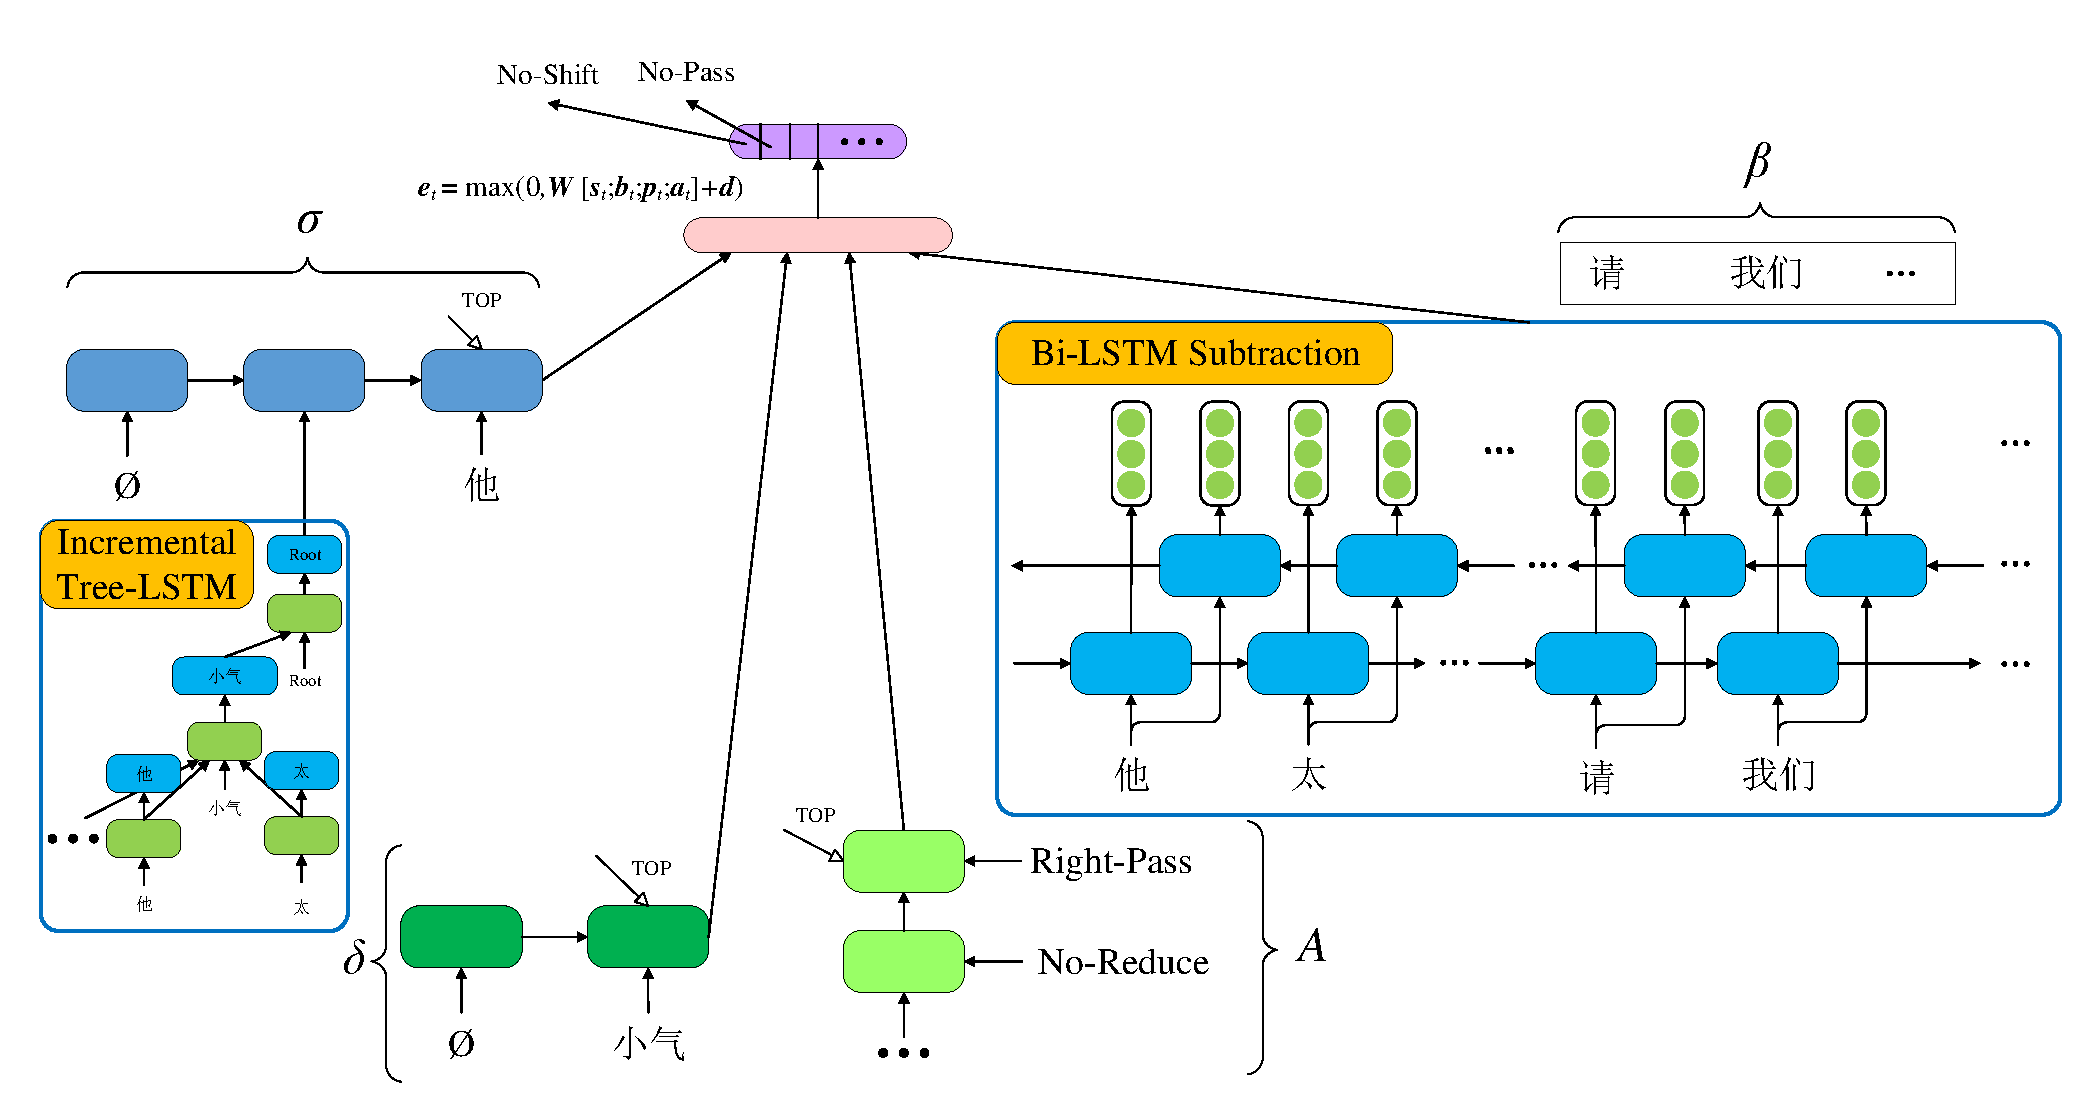
\includegraphics[width=0.9\textwidth]{figures/bs-it.pdf}
	\bicaption[fig:bs-it]{}{BS-IT系统模型整体结构图}{Fig.$\!$}{Model structure of BS-IT system}
\end{figure}

原始的Stack-LSTM中简单地使用从右向左的单向LSTM的最后一个隐层状态向量表示列表中的所有信息。
这种方法不但无法获取列表之外的词(已被移入栈中或规约)的信息,也损失了从左向右的上下文信息。
而且,只使用最后一个隐层状态向量难以很好地表示整个列表中的信息。

Wang和Cross等人探索了使用LSTM两个时间节点的隐层输出之差表示这两个节点中间的一段信息的方式,证明了该方法的有效性。\cite{wang-chang-2016-graph,cross-huang-2016-span}
类似的,本章提出Bi-LSTM Subtraction模块,将列表看作一个段,并用段头和段尾的隐状态之差来表示整个段。
因此,为了获得列表之外词的信息,该方法首先将整个句子输入双向LSTM中,用每个词对应的隐层状态向量作为其表示。

具体来说,整个列表在$t$时刻的表示$\bm{b}_t$:
\begin{equation}
	\bm{b}_f=\bm{h}_{f(l)}-\bm{h}_{f(r)}
\end{equation}
\begin{equation}
	\bm{b}_b=\bm{h}_{b(r)}-\bm{h}_{b(l)}
\end{equation}
\begin{equation}
	\bm{b}_t=[\bm{b}_f ; \bm{b}_b]
\end{equation}
其中,$l$和$r$分别表示在$t$时刻列表$\beta$中最左边的词和最右边的词,$\bm{h}_{f(a)}$和$\bm{h}_{b(a)}$分别表示词$a$在从左向右和从右向左的LSTM中的隐层输出。

\begin{figure}[hbtp]
	\centering
	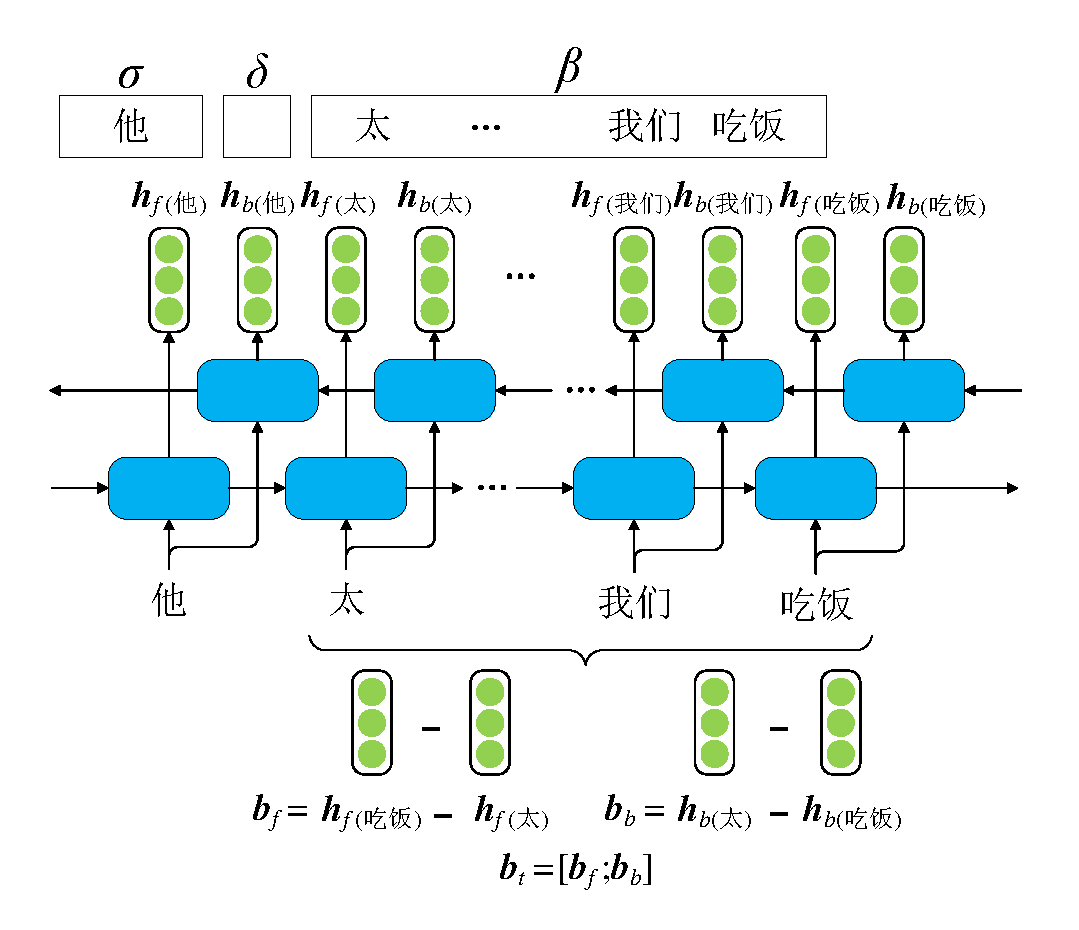
\includegraphics[width=0.7\textwidth]{figures/bs.pdf}
	\bicaption[fig:bs]{}{Bi-LSTM Subtraction模块结构图}{Fig.$\!$}{Model structure of Bi-LSTM Subtraction}
\end{figure}

图\ref{fig:bs}中给出了使用Bi-LSTM Subtraction模块计算列表的表示的例子。
首先使用“吃饭”的正向LSTM隐状态$\bm{h}_{f(\text{吃饭})}$减去“太”的正向LSTM隐状态$\bm{h}_{f(\text{太})}$,获得该段正向的表示向量,再用“太”的反向LSTM隐状态$\bm{h}_{b(\text{太})}$减去“吃饭”的反向LSTM隐状态$\bm{h}_{b(\text{吃饭})}$,获得该段反向的表示向量。
二者拼接起来作为此时列表的表示。

此外,原始的Stack-LSTM模型中使用基于依存的递归神经网络来计算转移过程中的子结构,在处理较深的子结构时,这种方法可能会遇到梯度消失问题。
为了解决该问题,本章在Tree-LSTM的基础上提出Incremental Tree-LSTM模块对这些子结构进行建模。
图\ref{fig:it}显示了本章提出的Incremental Tree-LSTM与基于依存的递归神经网络的区别。
递归神经网络通过递归地组合一个个父节点-子节点对来构建子图,而Tree-LSTM则能同时合并一个节点及其所有子节点。

由于基于转移的依存图分析的特点,本章中使用的Tree-LSTM与一般的Tree-LSTM有两点不同。
首先,该任务中需要建模的子结构不一定是树。
但由于需要处理的依存图不包括环,因此仍然能够使用LSTM。
更重要的是,与一般的Tree-LSTM能够同时获得一个节点的所有子节点不同,在基于转移的依存分析中,一个节点的子节点是逐个被找到的。
因此在Incremental Tree-LSTM中,需要不断利用Tree-LSTM更新父节点信息。
具体来说,对于一个词,每当找到它的一个新子节点,就要将其所有已经找到的子节点和其本身的表示输入Tree-LSTM中计算它的新表示。

\begin{figure}[hbtp]
	\centering
	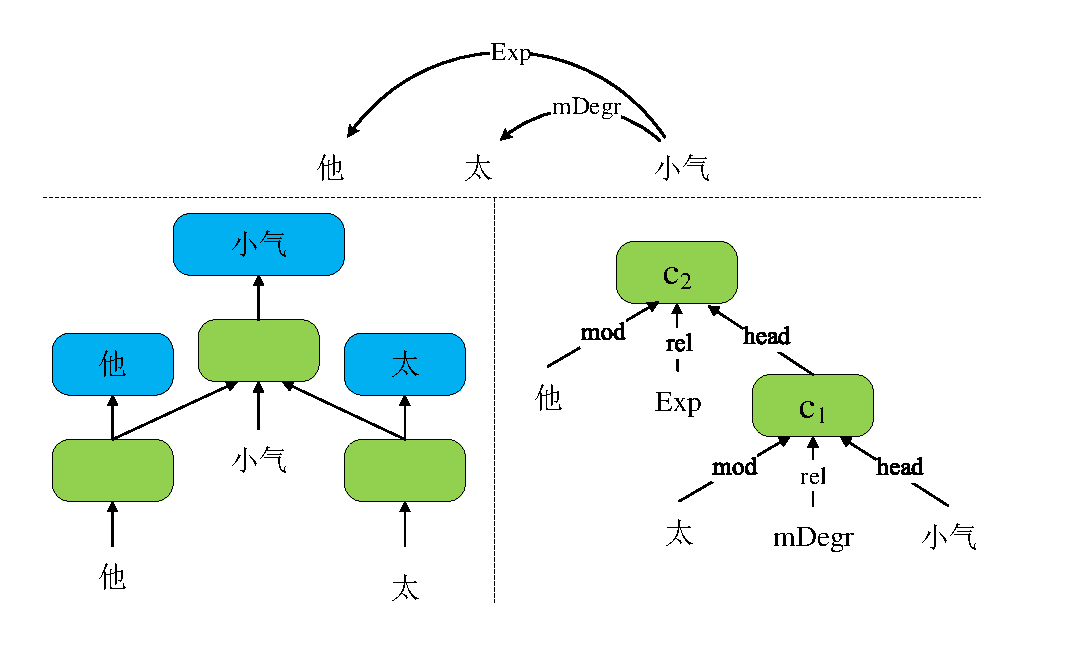
\includegraphics[width=0.8\textwidth]{figures/it.pdf}
	\bicaption[fig:it]{}{Incremental Tree-LSTM模块(左)与递归神经网络(右)对比图}{Fig.$\!$}{Comparison between Incremental Tree-LSTM and recursive neural network.}
\end{figure}

图\ref{fig:it}中给出了Incremental Tree-LSTM模块与递归神经网络在建模同一个子图时的对比图。
在转移过程中,“太”与“小气”之间的依存弧首先被生成,这时需要用Tree-LSTM合并二者的表示向量并将其作为“小气”的新表示。
在递归神经网络中,这一步的处理方法与Incremental Tree-LSTM模块基本相同,都是先合并“太”和“小气”的表示向量。
在第二步中,“小气”与其另一个子节点“他”之间的依存弧被生成,这时在Incremental Tree-LSTM模块中需要用Tree-LSTM合并“他”和“小气”的表示,以及之前已经找到的“小气”的子节点“太”的表示,将这三者表示合并之后作为父节点“小气”的新表示。
而在递归神经网络中,这一步则只需要合并“他”的表示向量之前已经生成的“太”和“小气”合并后的表示向量。
另外,值得注意的是,在Incremental Tree-LSTM模块中没有建模依存弧上的依存关系类别,而在递归神经网络中则建模了这一信息。
本章针对该问题使用原始Stack-LSTM模型进行了初步试验,发现从递归神经网络中删除依存关系类别信息并不会对最终结果产生太明显的影响。

\begin{figure}[hbtp]
	\centering
	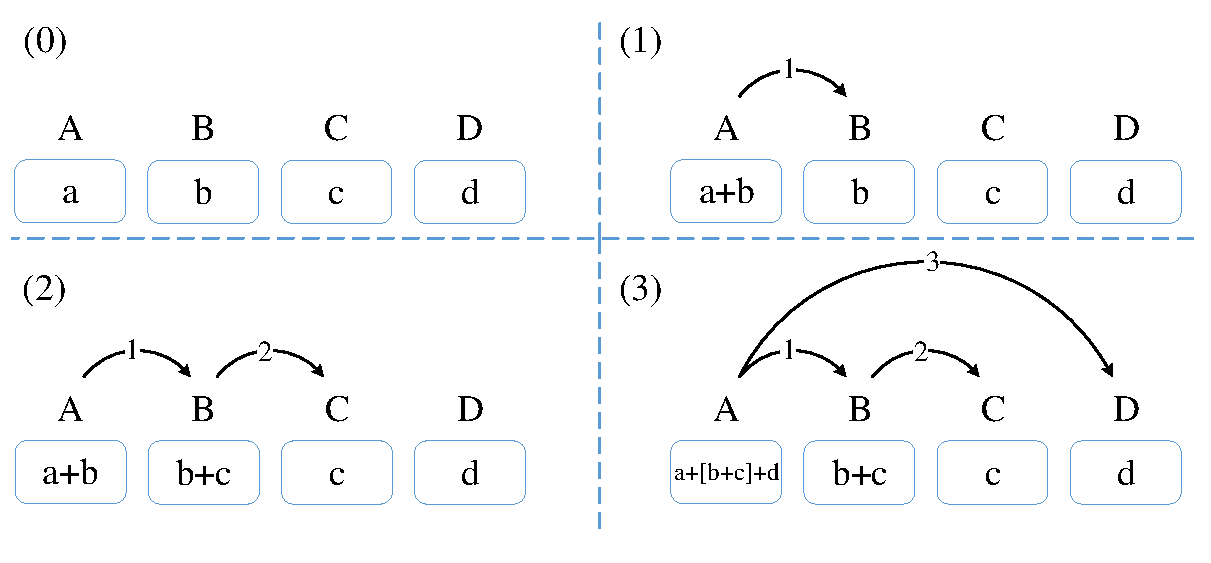
\includegraphics[width=0.8\textwidth]{figures/it-example.pdf}
	\bicaption[fig:it-example]{}{Incremental Tree-LSTM模块更新示例}{Fig.$\!$}{Example of updating in Incremental Tree-LSTM module.}
\end{figure}

为了进一步说明Incremental Tree-LSTM模块中根据当前生成的依存弧逐步更新Tree-LSTM状态的方式,图\ref{fig:it-example}给出了一个基于转移的依存分析中逐步生成的子图在Incremental Tree-LSTM模块中的更新过程的示例。
其中大写字母A、B、C、D表示句子中的词,小写字母a、b、c、d表示这些词对应的原始表示向量,而依存弧上的数字序号表示其生成的顺序。
该图中显示了以下4个状态:

1.初始状态下四个词之间还没有弧生成,这是他们的表示向量就是LSTM的隐层状态。

2.第一条由A指向B的依存弧生成后,A和B的表示向量a和b经过Tree-LSTM组合后代替A原来的表示向量。

3.第二条由B指向C的依存弧生成后,B和C的表示向量b和c经过Tree-LSTM组合后代替B原来的表示向量。

4.第三条由A指向D的依存弧生成后,A的原始表示向量a、B此时的表示向量b+c和D的表示向量d经过Tree-LSTM的组合后代替A原来的表示向量。

需要指出的是,在递归神经网络中,在第4步由A指向D的依存弧生成后,其只会直接将D的表示向量和A当时的表示向量(a+b)进行组合。
这样就遗漏了在前面的步骤中找到的B的子节点C的信息。
而在本章提出的Incremental Tree-LSTM模块中,这类信息则不会被遗漏。

\section{实验与分析}[Experiments and Analysis]

\subsection{实验设置}[Experimental Settings]

本章在中文和英文的语义依存图分析语料库上分别测试了BS-IT语义依存图分析模型的性能。
其中中文的语义依存图分析语料库来自SemEval-2016 Task 9\cite{che-etal-2016-semeval},是哈尔滨工业大学社会计算与信息检索研究中心和北京语言大学合作标注的中文语义依存图数据,其中按照句子来源分为两个子集,分别是新闻集(NEWS)和小学课本集(TEXT),前者句子较长、较复杂,后者句子较短、较简单。
而英文的语义依存图分析语料库来自SemEval-2015 Task 18\cite{oepen-etal-2015-semeval}英文广义语义依存图数据集。
该数据集一共有三种标注规范(DM、PAS和PSD),每种规范都有两部分测试数据集,即同领域(IN-DOMAIN)与异领域(OUT-OF-DOMAIN)测试数据。
中英文数据集的相关信息见表\ref{tbl:sdp-statistics}。
值得注意的是,由于DM、PAS和PSD是在相同的语料上按照不同的标注规范标注的,它们的各个集合的句子数是相同的,只有标签数量不同。

\begin{table}[htbp]
    \bicaption[tbl:sdp-statistics]{}{语义依存图语料库信息}{Table$\!$}{Statistics of Chinese semantic dependency graph dataset.}
    \vspace{0.5em}\centering\wuhao
    \begin{tabular}{ccccccc}
        \toprule[1.5pt]
        数据集 & 标签数 & 训练集 & 开发集 & 同领域测试集 & 异领域测试集 & 平均句子长度 \\
        \midrule[1pt]
        TEXT & 157 & 10,754 & 1,535 & 3,073 & 0     & 11.89 \\
        NEWS & 157 & 8,301  & 534   & 1,233 & 0     & 29.79 \\
        DM   & 61  & 33,964 & 1,692 & 1,410 & 1,849 & 22.26 \\
        PAS  & 43  & 33,964 & 1,692 & 1,410 & 1,849 & 22.26 \\
        PSD  & 92  & 33,964 & 1,692 & 1,410 & 1,849 & 22.26 \\
        \bottomrule[1.5pt]
    \end{tabular}
\end{table}

实验中使用的评测指标包括不计算弧标签的F值(UF)、计算弧标签的F值(LF)、有多父节点的词中不计算弧标签的F值(NUF)和有多父节点的词中计算弧标签的F值(NLF)。
其中值得注意的是NLF值,该指标只统计与有多个父节点的词相连的弧的计算标签的F值,也就是将目光集中在语义依存图分析中最难以解决的弧上,因此更能反映模型解决该问题的能力。

\subsection{实验结果}[Results]

\begin{table}[htpb]
    \bicaption[tbl:result-semeval16]{}{中文语义依存图数据集上的实验结果}{Table$\!$}{Results on Chinese semantic dependency graph dataset.}
	\centering
	\small
	\renewcommand{\arraystretch}{1.2}
	\begin{tabular}{l|cccc|cccc}
		\hline
		\multirow{2}{*}{ 系统}&\multicolumn{4}{c}{NEWS}&\multicolumn{4}{c}{TEXT}\\
		\cline{2-9}
		& LF& UF& NLF& NUF& LF& UF& NLF& NUF\\
		\hline
		IHS-RD-Belarus&59.06&77.64&40.84&60.20&68.59&82.41&50.57&64.58\\
		OCLSP (lbpg)&57.22&74.93&45.57&58.03&65.54&79.39&51.75&63.21\\
		OCLSP (lbpgs)&57.81&75.54&41.56&54.34&66.21&79.85&47.79&55.51\\
		OCLSP (lbpg75)&57.78&75.40&48.89&58.28&66.38&79.91&57.51&63.87\\
		OSU\_CHGCG&55.69&73.72&49.23&60.71&65.17&78.83&54.70&65.71\\
		MLP & 60.71&77.86&47.01&61.90&70.04&82.01&55.59&65.55 \\ 
		Two-Stage & 62.29&80.56&39.93&64.29&71.94&85.24&50.67&69.97 \\ 
		Stack-LSTM &62.23&80.42&49.18&63.90&71.51&84.95&59.70&71.63\\
		BS-IT &\bf63.30&\bf81.14&\bf51.16&\bf66.92&\bf72.92&\bf85.71&\bf61.91&\bf72.74\\
		\hline
	\end{tabular}
\end{table}

表\ref{tbl:result-semeval16}中列出了中文语义依存图数据集上的实验结果。
下面分别介绍表中所列的各个基线模型:
\begin{itemize}
    \item IHS-RD-Belarus:
    \item OCLSP:
    \item OSU\_CHGCG:
    \item MLP:
    \item Two-Stage:该模型是我们参考Ding等人\cite{ding-etal-2014-dependency}于2014年提出的方法重新实现的基线模型。其中首先用传统依存树分析器预测出依存树结构,然后用一个支持向量机(Support Vector Machine,简称SVM)作为分类器从一个由规则产生的候选弧集合中选出一些弧加入其中组合成语义依存图。
    \item Stack-LSTM:
\end{itemize}

表中前5行是参加SemEval-2016 Task 9评测的其它系统的结果。
第6行是我们录用于CCL 2016的论文中使用MLP作为分类器的系统的结果。
最后两行是我们录用于AAAI 2018的论文中提出了模型,其中Basic表示不使用Bi-LSTM Subtraction和Incremental Tree-LSTM两个模块时的结果,BS-IT表示同时使用这两个模块时的结果。
实验结果显示我们提出的模型获得了该数据集上最好结果,尤其在对图结构评价至关重要的NLF值上相比原有方法有巨大提升。

\begin{table}[htpb]
    \bicaption[tbl:result-semeval15]{}{英文语义依存图数据集上的实验结果}{Table$\!$}{Results on English semantic dependency graph dataset.}
	\centering
	\small
	\renewcommand{\arraystretch}{1.2}
	\begin{tabular}{l|ccc|c}
		\hline
		\bf 系统&\bf DM&\bf PAS&\bf PSD &\bf 宏平均\\
		\hline
		\multicolumn{5}{c}{\bf IN-DOMAIN}\\
		\hline
		Du 15 (ensemble) &89.1&91.3&75.7&85.4\\
		Almeida 15 (single) &88.2&90.9&76.4&85.2\\
		Peng 17 (single) &89.4&\bf 92.2&77.6&86.4\\
		\hline
		BS-IT (single) &89.3&91.4&76.1&85.6\\
		BS-IT (ensemble) &\bf 90.3& 91.7&\bf 78.6&\bf 86.9\\
		\hline
		\multicolumn{5}{c}{\bf OUT-OF-DOMAIN}\\
		\hline
		Du 15 (ensemble) &81.8&87.2&73.3&80.8\\
		Almeida 15 (single) &81.8&86.9&74.8&81.2\\
		Peng 17 (single) &84.5&\bf 88.3&75.3&82.7\\
		\hline
		BS-IT (single) &83.2&87.2&73.2&81.2\\
		BS-IT (ensemble) &\bf 84.9&87.6&\bf 75.9&\bf 82.8\\
		\hline
	\end{tabular}
\end{table}

表\ref{tbl:result-semeval15}中列出了英文语义依存图数据集上的实验结果,其中所列均为LF值,single表示单模型方法,ensemble表示多模型融合方法。
下面分别介绍表中所列的各个基线模型:
\begin{itemize}
    \item Du 15 \cite{du-etal-2015-peking} :该模型由Du等人于2015年提出,其中利用了多个不同的基于转移和基于图的模型同时预测并对最终结果进行投票。
    \item Almeida 15 \cite{almeida-martins-2015-lisbon}:该模型由Almeida等人于2015年提出,其中使用了基于图的依存分析方法,利用了$AD^3$算法进行解码。
    \item Peng 17 \cite{peng-etal-2017-deep}:该方法由Peng等人于2017年提出,他们使用一个基于图的方法,同时利用三种标注体系进行多任务学习,取得了该数据集上当时最好结果。这里列出的是他们没有使用多任务学习的基础模型结果。
\end{itemize}

BS-IT是我们的系统结果。此外,我们也使用了一个简单的模型融合方法,在训练时使用不同随机初始化种子训练多个模型。在预测时,用这些模型算出的分数之和来选择接下来的转移动作。实验证明该方法有效提高了系统性能,从而达到与该数据集上最好结果相近的结果。



\section{本章小结}[Conclusions]


% Local Variables:
% TeX-master: "../thesis"
% TeX-engine: xetex
% End: